\documentclass[24pt,margin=20mm,innermargin=-6in,blockverticalspace=-0.25in]{tikzposter}
\geometry{paperwidth=46in,paperheight=33in}
\usepackage[utf8]{inputenc}
\usepackage{amsmath}
\usepackage{amsfonts}
\usepackage{amsthm}
\usepackage{amssymb}
\usepackage{mathrsfs}
\usepackage{graphicx}
\usepackage{caption}
\usepackage{subcaption}
\usepackage{adjustbox}
\usepackage{enumitem}
\usepackage{wrapfig}
\usepackage[backend=bibtex,style=numeric,doi=false,url=false,eprint=false,sorting=none]{biblatex}
\usepackage{uofa-theme}
\usetikzlibrary{positioning,shapes,arrows}


\addbibresource{ref.bib}
\AtBeginBibliography{\footnotesize}

% set theme parameters
\tikzposterlatexaffectionproofoff
\usetheme{UofATheme}
\usecolorstyle{UofAStyle}

\title{GRAVI: Gene Regulatory Analysis Using Variable Inputs}
\author{\centering \textbf{Stevie Pederson}\textsuperscript{1,2}, Geraldine Laven-Law\textsuperscript{1}, Richard Iggo\textsuperscript{1,3}, Amy Dwyer\textsuperscript{1}, Theresa E Hickey\textsuperscript{1} and Wayne D Tilley\textsuperscript{1}}
\institute{
  \textsuperscript{1}Dame Roma Mitchell Cancer Research Laboratories, Adelaide Medical School, University of Adelaide\\
  \textsuperscript{2}Black Ochre Data Labs, Telethon Kids Institute\hspace{5mm}
  \textsuperscript{3}Bordeaux Institute of Oncology, University of Bordeaux
}
%\titlegraphic{\includegraphics[width=0.1\textwidth]{UoA-standard-vert-rgb.jpg}}


% begin document
\begin{document}
\maketitle

\node [below right=20mm and 10mm] at (bottomleft |- topright) {
\includegraphics[width=0.08\textwidth]{UoAlogo.png}};
\node [below left=20mm and 10mm] at (topright) {
\includegraphics[width=0.08\textwidth]{tki.jpg}};



\centering

\block{GRAVI Outline}{
	\begin{minipage}{0.93\linewidth}
	\LARGE
	\textbf{GRAVI} is a \texttt{snakemake}\cite{Molder2021-mo} workflow for performing high-quality ChIP-Seq analysis.
	GRAVI standardises multiple steps to enable a \textit{complete standalone analysis}, as well as enabling \textit{integration across multiple cell types}.
	The minimal required data is a single ChIP target under 2 conditions expanding to \textit{any number of ChIP targets and conditions}.
	Optional RNA-Seq and HiC data further extend GRAVI to \textbf{directly map dynamic changes in ChIP signal to regulatory targets}.	
	\end{minipage}
	\begin{minipage}{0.06\linewidth}
		\begin{flushright}
	       	
\includegraphics[width=0.9\linewidth]{gravi-qr-code}		
		\end{flushright}  
	\end{minipage}
	\vspace{1cm}
}

\begin{columns}
    \column{0.31}
    	\block{Key Aims}{
%  	    	\begin{minipage}{0.25\linewidth}
%	       	\begin{flushleft}
%       		
\includegraphics[width=0.9\linewidth]{gravi-qr-code}
%       		\vspace{15mm}	       	
%	       	\end{flushleft}
%       	\end{minipage}
%    		\begin{minipage}{0.75\linewidth}
			\Large
		    \begin{enumerate}
		    \item Best Practice Differential ChIP Signal Analysis
		    \item Accurate Mapping of Binding Sites to Regulatory Targets
		    \item Integration of multiple ChIP targets \& treatments
		    \item Highly flexible input data
		    \end{enumerate}    		
%    		\end{minipage}

    	}
    	\block{Input Data}{
    	    \large
    		\begin{minipage}{0.42\linewidth}
    		\innerblock{Required Input}{
	    		\begin{itemize}
	    		\item $1\times$ChIP Target (.bam)
	    		\begin{itemize}
	    			\item $2\times$ Conditions	    		
	    		\end{itemize}
	    		\item Gene Annotations (.gtf) 
	    		\item Blacklisted Regions (.bed)
	    		\end{itemize}
	    		
	    	}    	
	    	\vspace{15mm}	
    		\end{minipage}
    		\begin{minipage}{0.58\linewidth}
    		\innerblock{Optional Input}{
    			\begin{itemize}
    			\item Additional ChIP targets/treatments
    			\item Differential Gene Expression (.tsv)
    			\item HiC Interactions (.bedpe)
    			\item Features of Interest (.gtf)
    			\item External Coverage Tracks (.bw)
    			\end{itemize}   		
    			}
    		\end{minipage}
    	}
    	\block{GRAVI Steps}{
		\Large
   		\begin{minipage}{0.52\linewidth}
	    		\innerblock{Always Performed}{
	    		\begin{enumerate}
%			\item Prepare Annotations
			\item Peak Calling and Sample QC
			\item Differential Signal Analysis
	    		\end{enumerate}
	    		}
    		\end{minipage}
   		\begin{minipage}{0.47\linewidth}
	    		\innerblock{Performed Only When Viable}{
	    		\begin{enumerate}[resume]
			\item Pairwise Comparisons
	    		\end{enumerate}
	    		}
    		\end{minipage}
    		
    	}

    	\block{Key Outputs}{
    		\Large
    		An extensive library of results for sharing with collaborators
    		
    		\begin{itemize}
    			\item Compiled Multi-Page HTML (Figures, Tables, Descriptions)
    			\item Bed Files (Peaks, Key Results)
    			\item BigWig Files (Visualisation)
    			\item Spreadsheets (Integrated results with mappings)
    			\item \texttt{R} Data Objects for Custom Downstream Analysis
    		\end{itemize}
    	}


    \column{0.36}
    \useblockstyle{KeyBlockStyle}
    \block{Motivation}{
    \Large
    Activation of the Androgen Receptor (AR) has \textit{anti-proliferative properties in many breast cancer models}\cite{Hickey2021}.
    Integrating the dynamics of AR binding with the Estrogen Receptor $\alpha$ (ER$\alpha$), additional transcription factors, H3K27ac marks and changes in transcription, we are able to investigate the underlying molecular mechanisms.
    Comparison across cancer models can then be used to identify key targets and mechanisms.
    }
    \useblockstyle{UofABlockStyle}
    
%   	\block{Annotation Preparation}{
%    A set of \textit{non-overlapping genomic regions} is defined for the specific annotations utilised, and incorporating all \textbf{transcript-level} information with genomic distances defined by the user.
%    Regions are defined as 1) Promoter, 2) Upstream Promoter, 3)Exon, 4) Intron, 5) Proximal Intergenic, and 6) Distal Intergenic.
%    The relationship between defined regions and any provided genomic features (e.g. H3K27ac) data or any long-range interactions (e.g. HiC) is also assessed.
%    Standardised colour schemes are also defined for propagation through the workflow.
%    }
    
%    \block{Peak Calling}{
%    	
%    	Macs2 callpeak\cite{macs2} is used for identifying peaks within individual replicates and across all replicates within a treatment group.
%    	QC on each sample is performed identifying using common metrics such as FRIP with the relationship between all samples assessed using UpSet Plots and VennDiagrams.
%    	Consensus peaks are identified with treatment groups and across all samples with all regions exported as \texttt{bed} files.\\[-5mm]
%    	
%        \begin{tikzfigure}[Example outputs for ER binding showing all samples as an UpSet plots, common consensus peaks  and the genomic distribution.]
%        	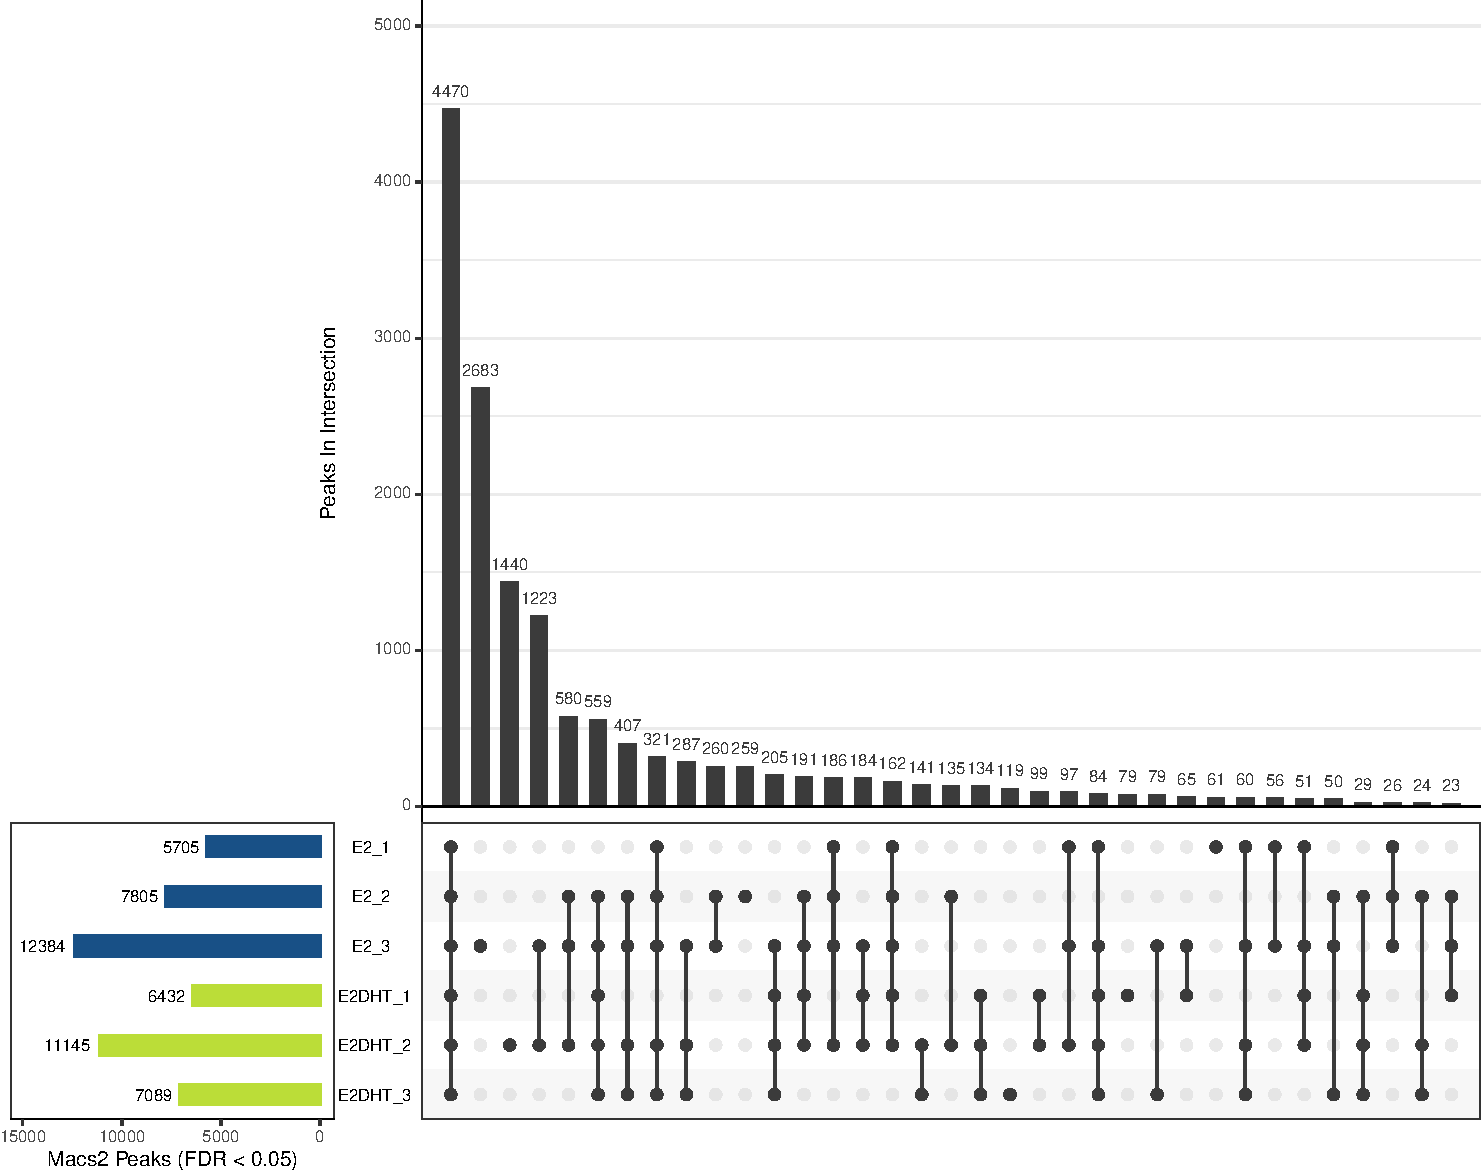
\includegraphics[width=0.35\linewidth]{all-reps-upset-1}
%        	\hfill
%        	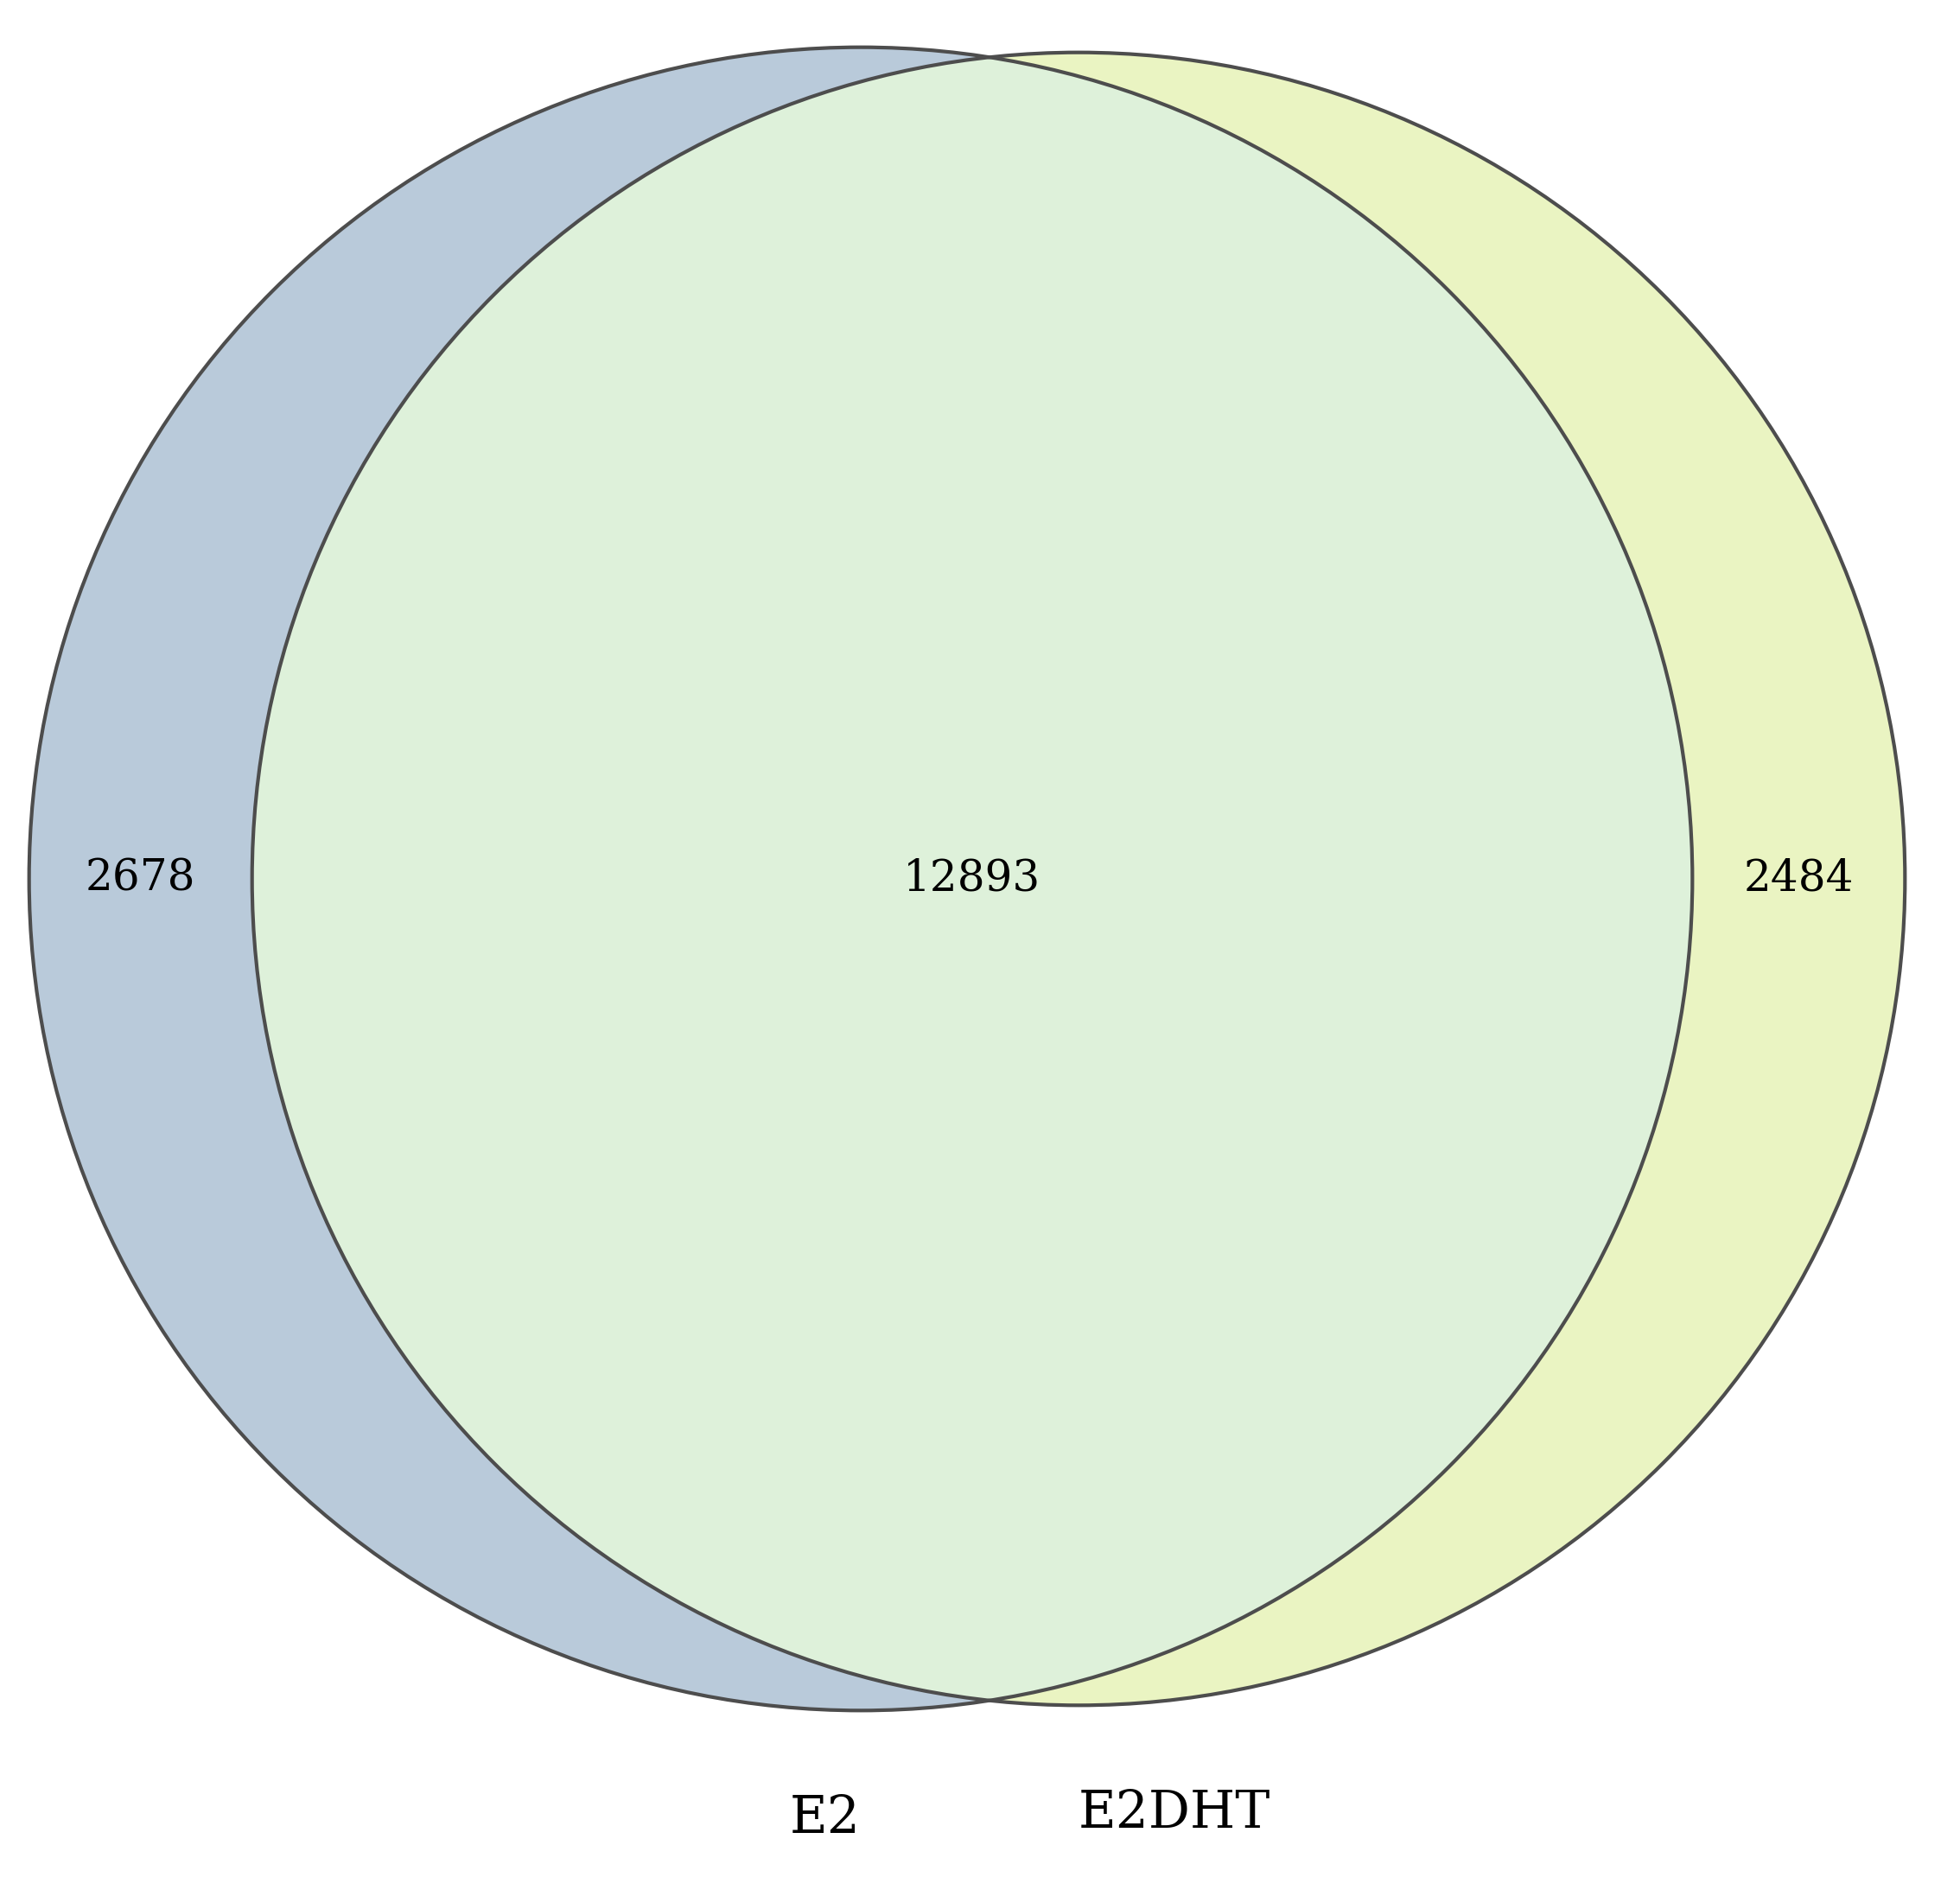
\includegraphics[width=0.25\linewidth]{ER_common_peaks}
%        	\hfill
%        	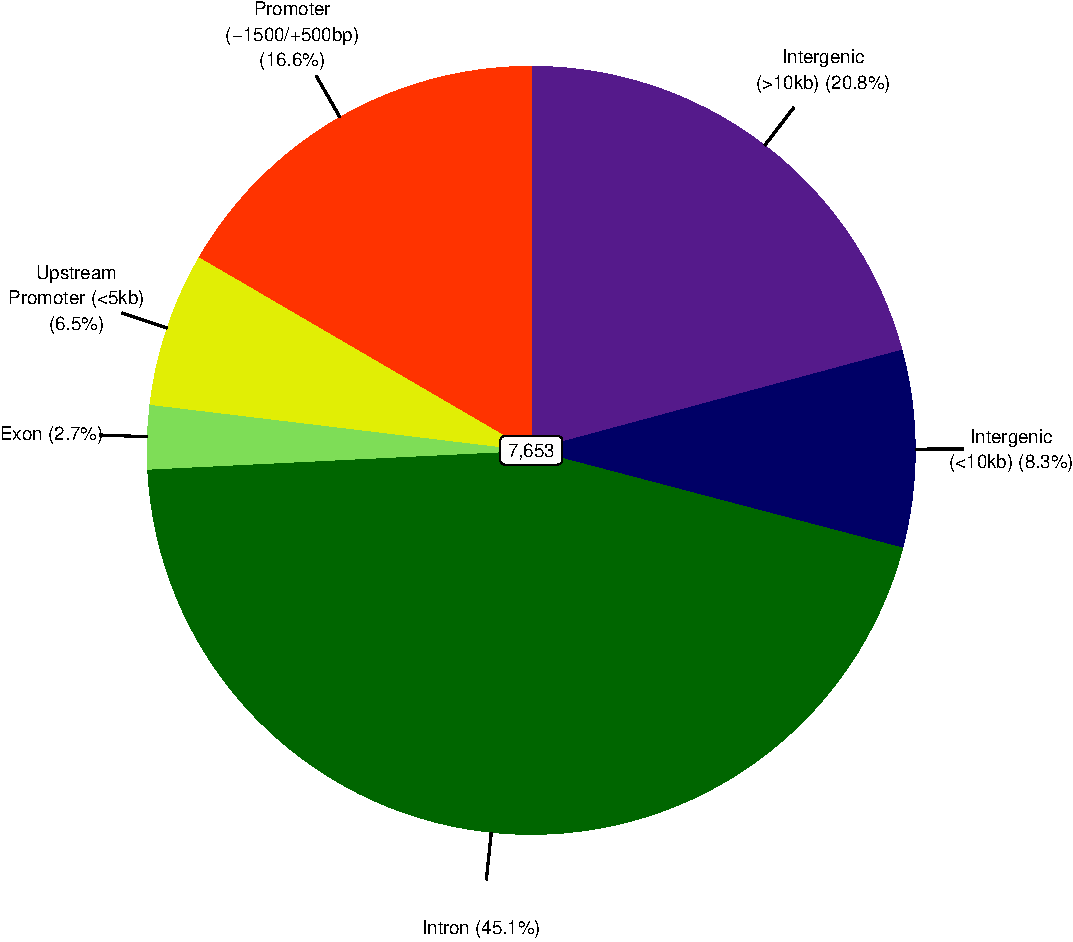
\includegraphics[width=0.3\linewidth]{plot-region-overlap-1}
%        \end{tikzfigure}
%    	
%    }

    \block{Differential Signal Analysis}{
    
	\begin{minipage}{0.45\linewidth}
		\innerblock{Consistent Steps}{
		    \begin{enumerate}
			    	\item Sliding Windows\cite{csaw} using 
			    	\begin{enumerate}
			    		\item Quasi-Likelihood Models\cite{Lund2012-xo}, or
			    		\item SQN\cite{sqn} with limma-trend\cite{voom}
			    	\end{enumerate}
			    	\item Range-Based $H_0$\cite{treat}
			    	\item Independent Hypothesis Weighting (IHW)\cite{Ignatiadis2016-cq}
			    	\item Mapped to Genes, Regulatory Regions and External Features
			    	\item Enrichment Analysis
			    	\begin{itemize}
			    		\item Tables and Network Plots
			    	\end{itemize}
			    	\item Multiple tables, figures and bed files
		    \end{enumerate}
		   }
		\innerblock{Steps With RNA-Seq}{
		    \begin{enumerate}
			    	\item Direct Targets Identified
			    	\item \textit{Combined} Enrichment Analysis
			    	\begin{itemize}
			    		\item Tables and Network Plots
			    	\end{itemize}
		    \end{enumerate}
		   }
		\innerblock{To Be Implemented Next}{
		    \begin{enumerate}
			    	\item Alternative Fixed-Width Analysis
			    	\item TMM/RLE Normalisation
			    	\item ATAC-Seq Methods
		    \end{enumerate}
		   }
%	\vspace{5cm}
	\end{minipage}	    
	\begin{minipage}{0.55\linewidth}
	
		\centering
    		\begin{tikzfigure}[AR logCPM values before and after Smooth Quantile Normalisation. AR is primarily cytoplasmic then shifts to be nuclear under E2+DHT\label{fig:logCPM}]
        	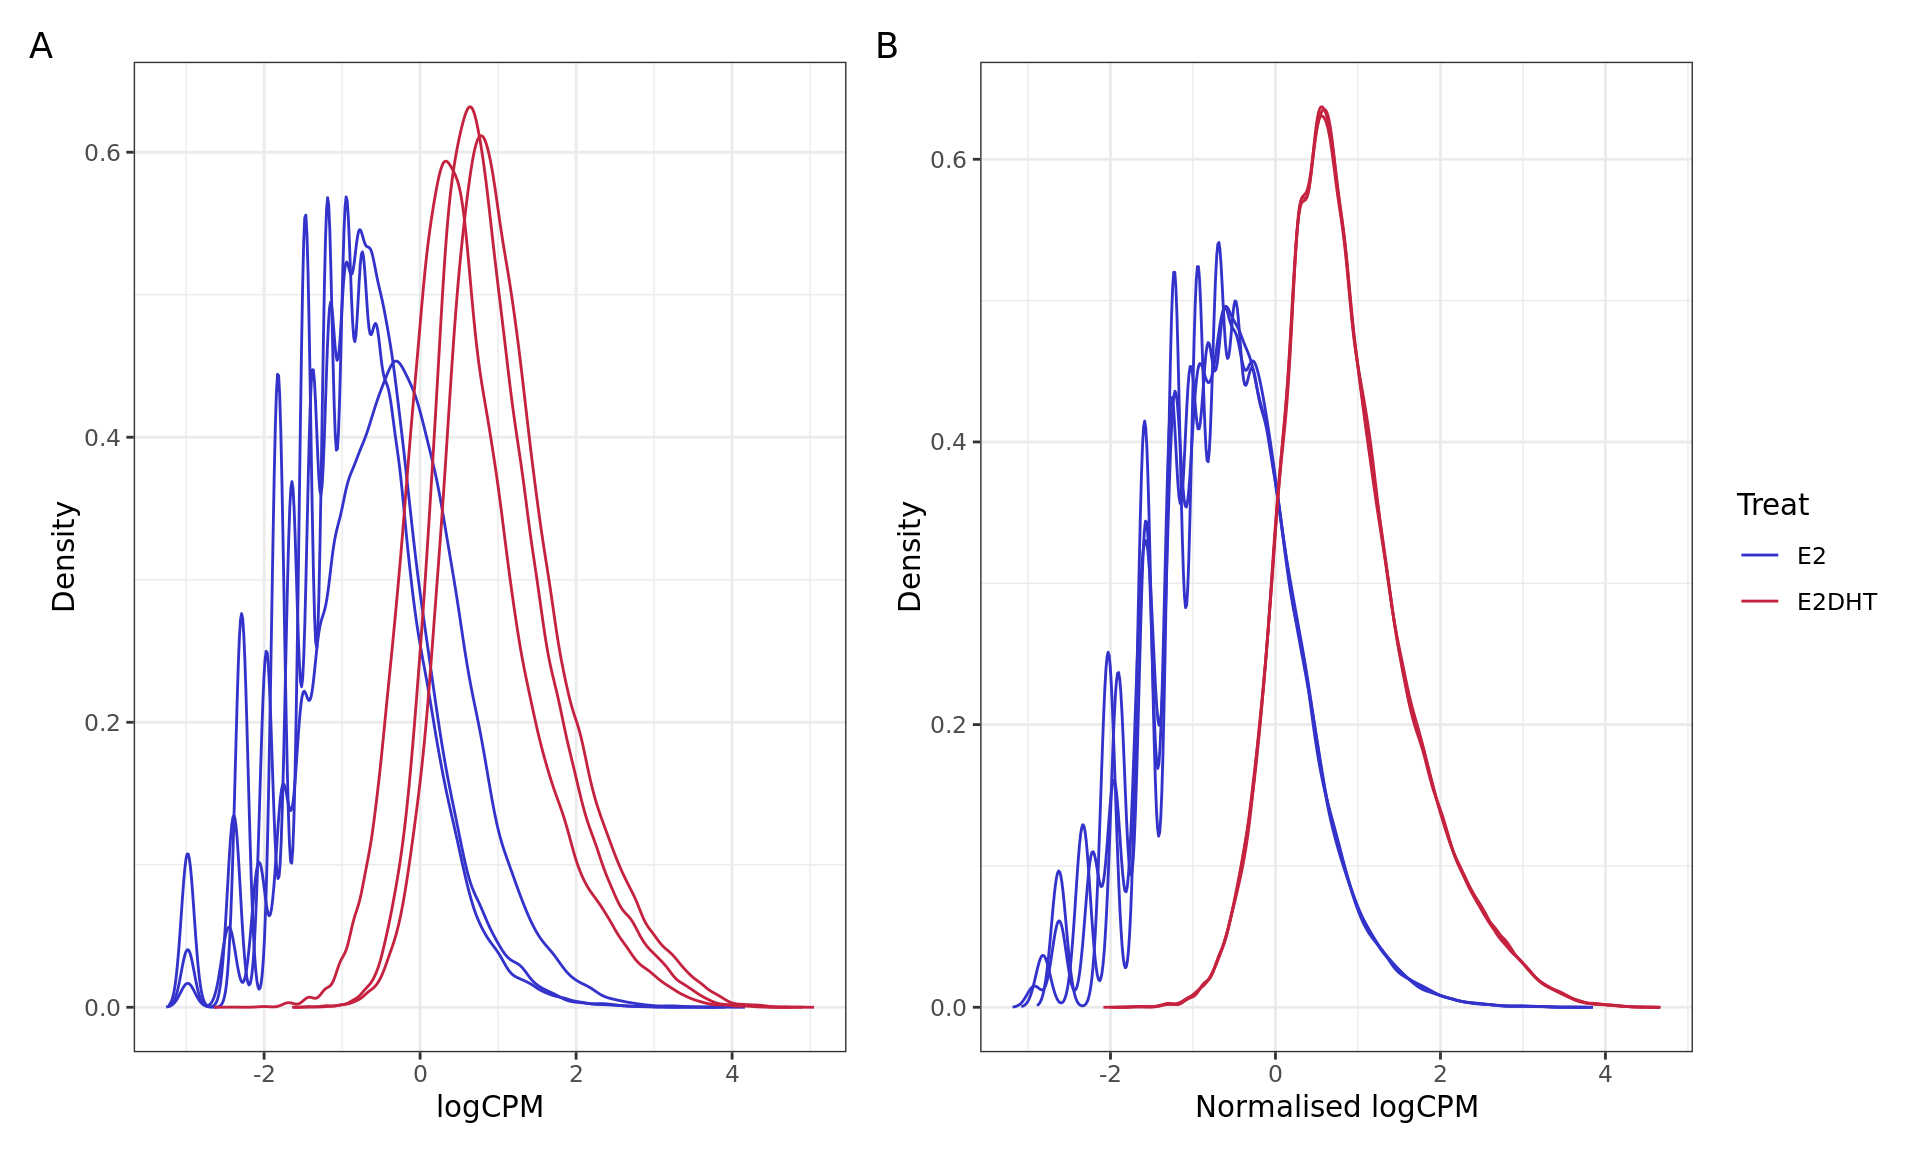
\includegraphics[width=0.98\linewidth]{ar-logcpm-densities-1}
        \end{tikzfigure}		
        
           \begin{tikzfigure}[Partitioned p-values for H3K27ac signal based on co-detection of AR and ER.\label{fig:ihw}]
	        	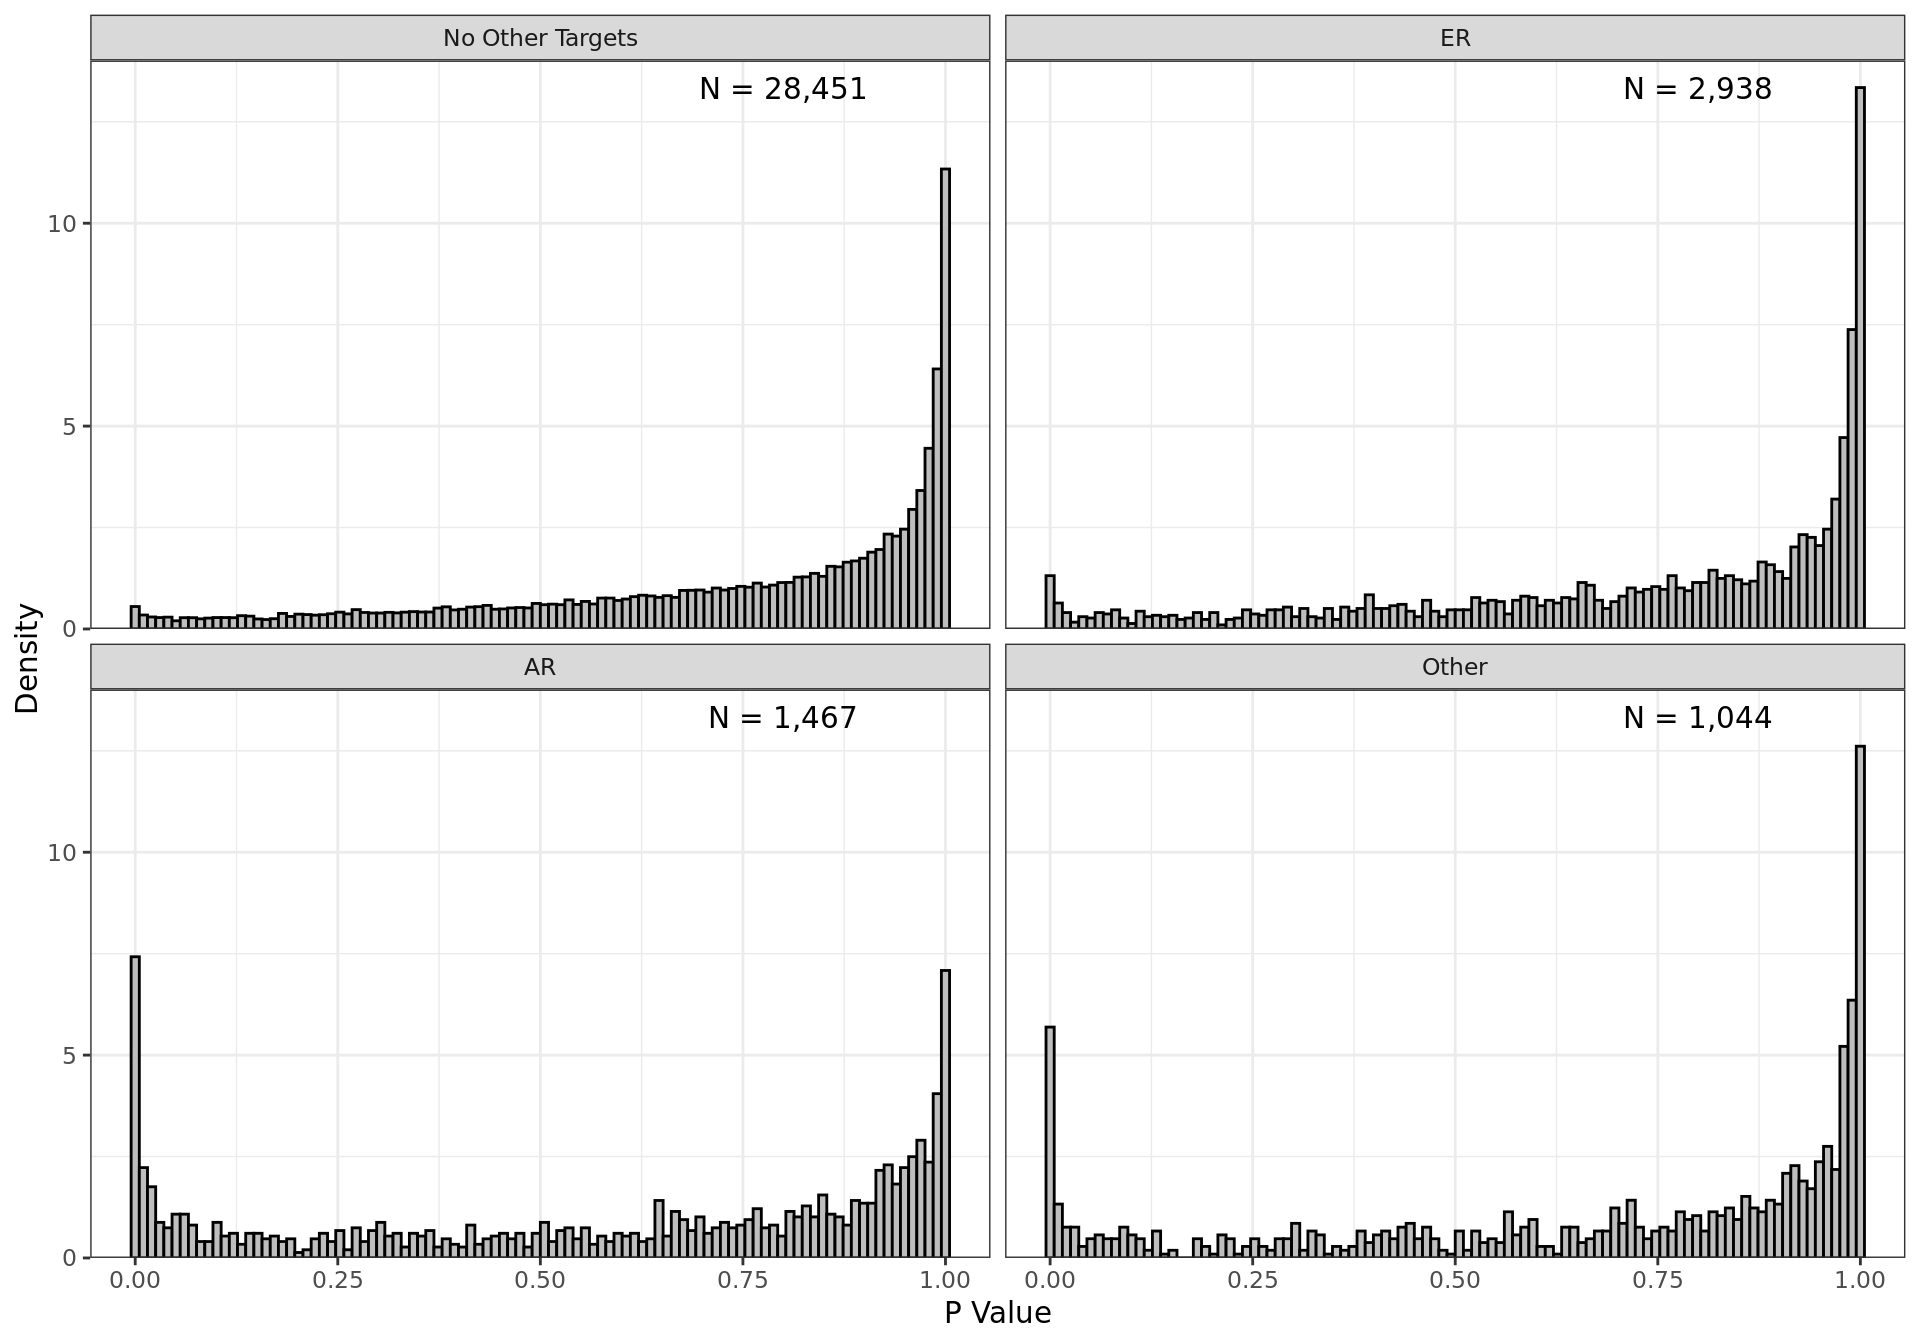
\includegraphics[width=0.98\linewidth]{h3k27ac-ihw-pvals-1}
    	    \end{tikzfigure}	
        
	\end{minipage}    	

%  		\begin{minipage}{0.5\linewidth}
%  			\centering
%           \begin{tikzfigure}[Partitioned p-values for the GATA3 binding response to DHT based on co-detection of the additional ChIP targets AR and ER.\label{fig:ihw}]
%	        	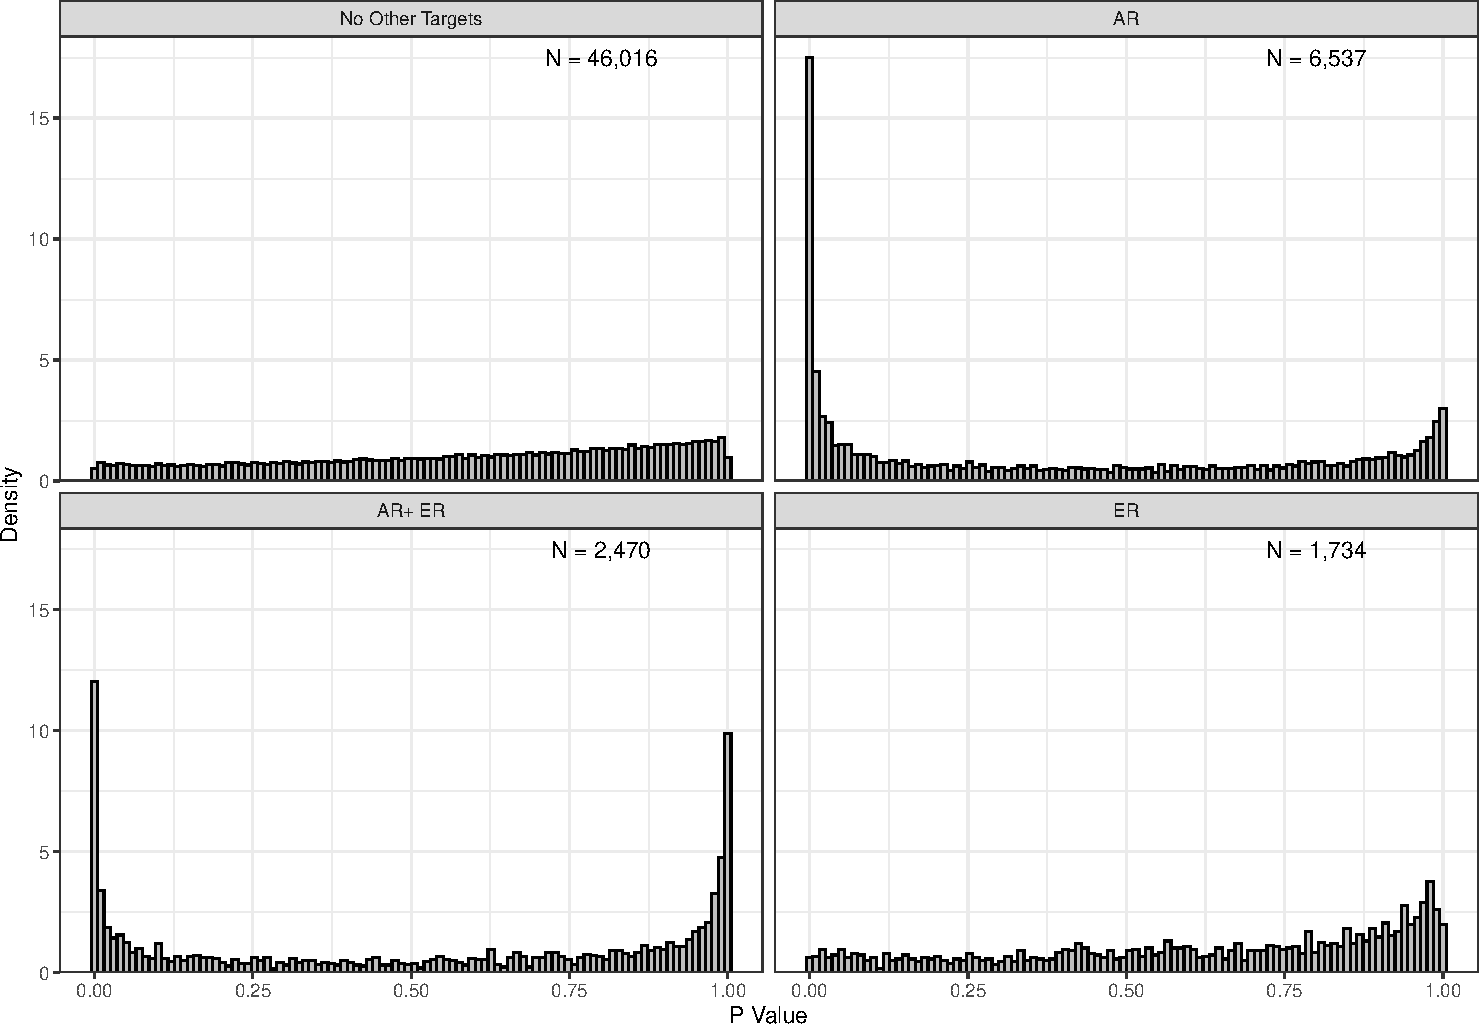
\includegraphics[width=0.8\linewidth]{plot-ihw-pvals-1}
%    	    \end{tikzfigure}	
%    	\end{minipage}
    	

    	
    }

    \column{0.32}
    \block{Pairwise Comparisons}{
		\begin{wrapfigure}{r}{0.16\linewidth}
			\centering
			
\includegraphics[width=0.9\linewidth]{extraChIPs_sticker}
		\end{wrapfigure}    
		Given prior rigour in statistical testing, comparison across pairs of factors becomes more of a \textit{site classification problem}.
		When a site is found to be responsive for one transcription factor a lower p-value threshold is applied to the second factor in any overlapping sites, ensuring \textbf{unchanged sites are classified more accurately} as these are important in a pairwise analysis.
		Each site is classified across both ChIP targets as \textit{Up, Down, Unchanged or Undetected} yielding a set of pairwise classifications.
		Comparisons of changed binding (Figure \ref{fig:pairwise-logfc}) are generated across all sites, and separated by annotated region or external feature.
		Profile heatmaps are also created (Figure \ref{fig:heatmap-ar-er}) and enrichment testing is performed on each set of regions.
		Example sites for each set of regions are also plotted by default using \texttt{extraChIPs::plotHFGC()} (Figure \ref{fig:zbtb16}).
		If RNA-Seq data is provided, an analysis of DE genes by pairwise changes in ChIP target binding is also performed (Figure \ref{fig:volcano}).\\
		
		
		\begin{minipage}{0.5\linewidth}
			\centering
           \begin{tikzfigure}[Pairwise logFC values for AR and ER broken down by externally provided H3K27ac-defined features.\label{fig:pairwise-logfc}]
	        	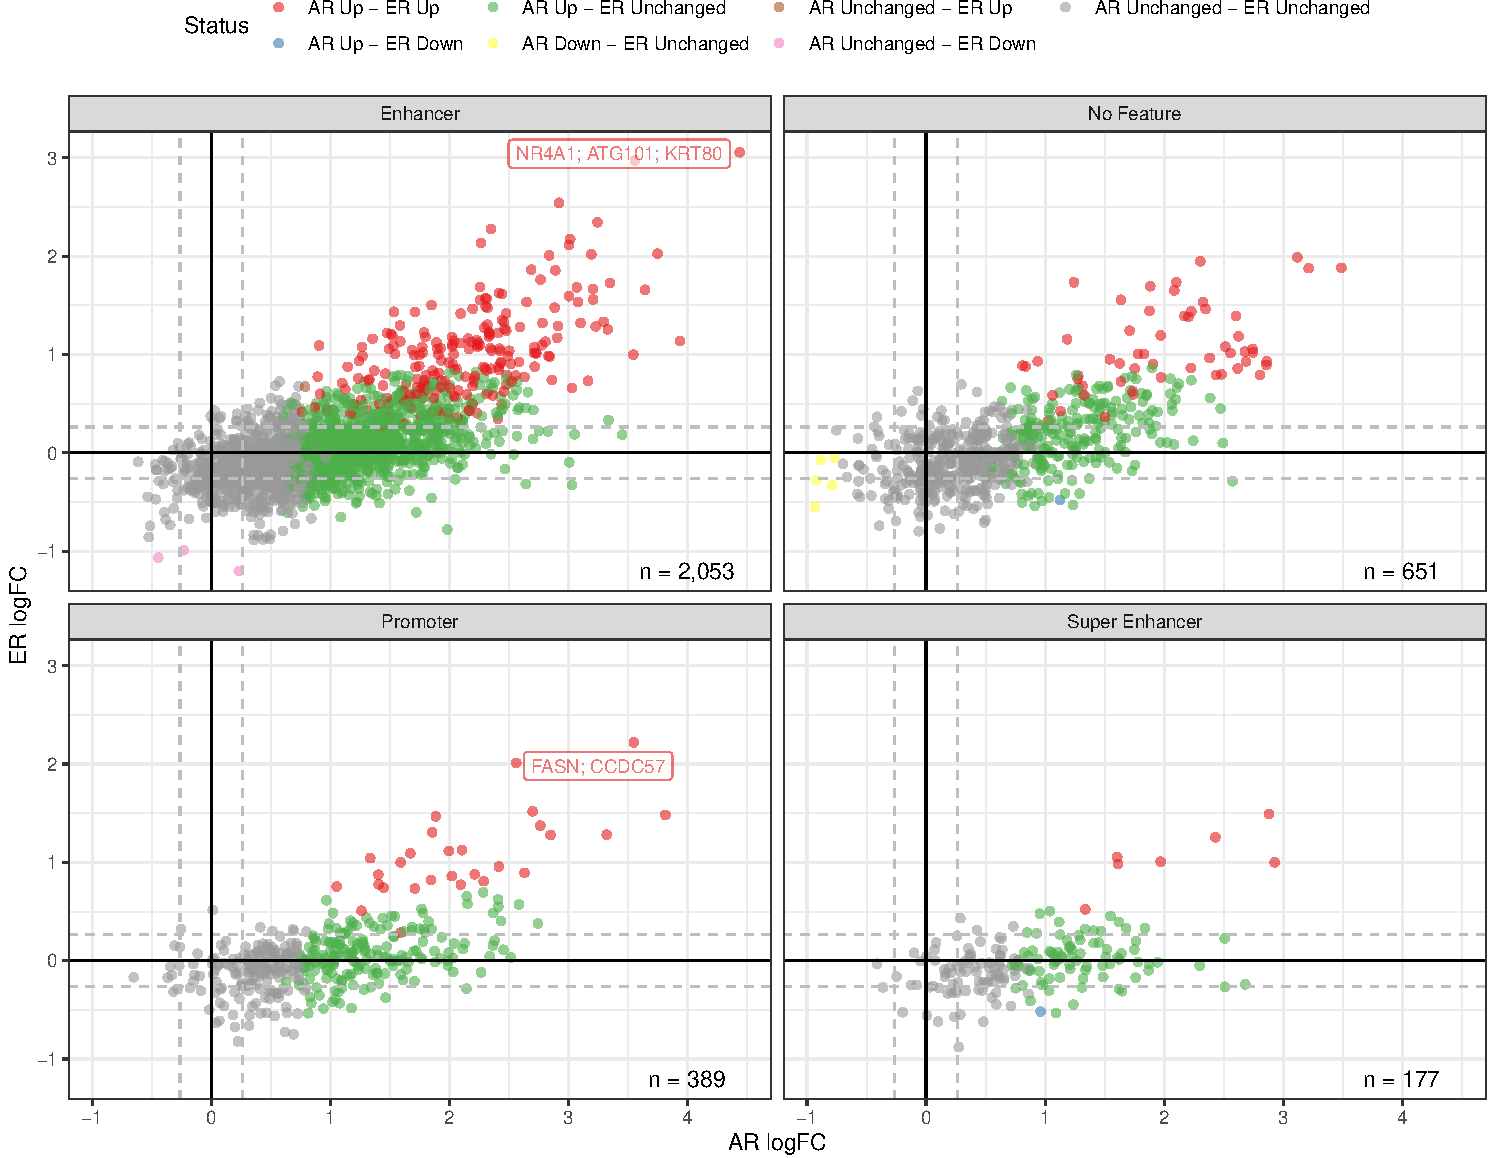
\includegraphics[width=0.9\linewidth]{plot-dbwin-by-feature-1}
    	    \end{tikzfigure}		
		\end{minipage}
  		\begin{minipage}{0.5\linewidth}
  			\centering
	    	\begin{tikzfigure}[Profile heatmap for sites showing increased binding for both AR and ER.\label{fig:heatmap-ar-er}]
	        	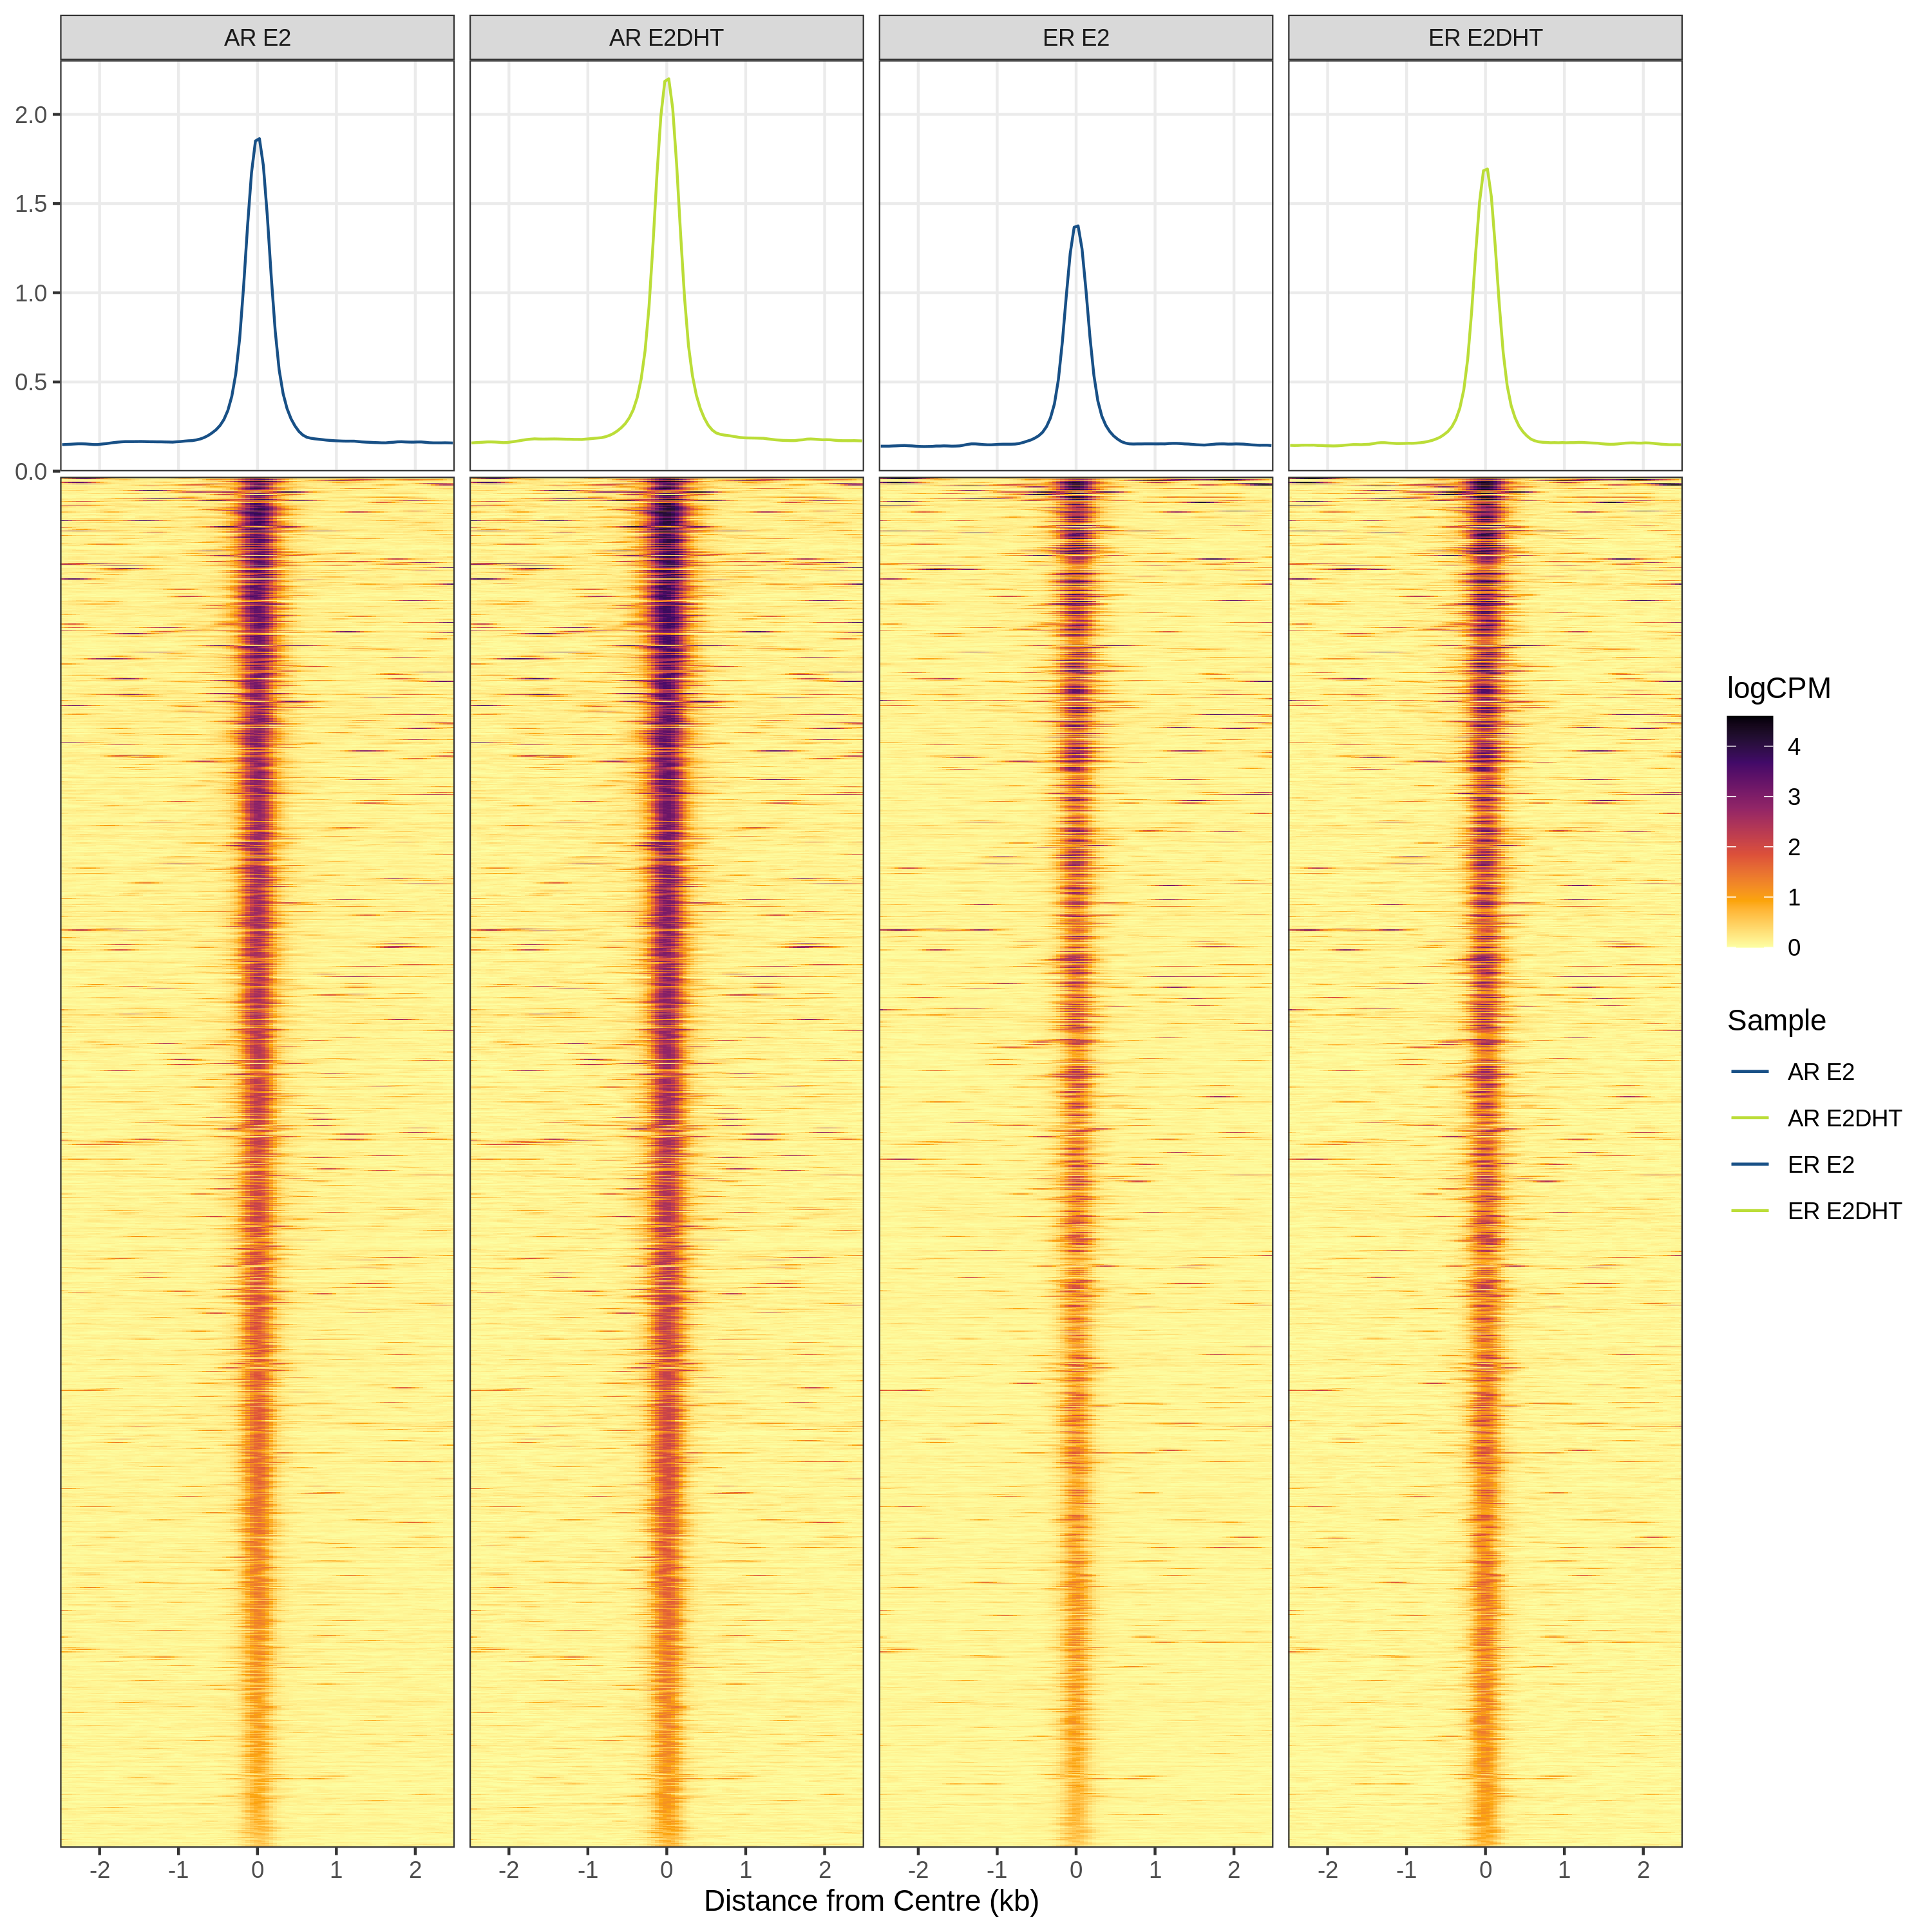
\includegraphics[width=0.7\linewidth]{AR_Up_ER_Up_profile_heatmap}
	        \end{tikzfigure}
    	\end{minipage}\\[8mm]
    	
		\begin{minipage}{0.5\linewidth}
			\centering
           \begin{tikzfigure}[\textit{ZBTB16} is up-regulated, shows increased binding for both AR and ER, with an increase in H3K27ac signal\label{fig:zbtb16}]
	        	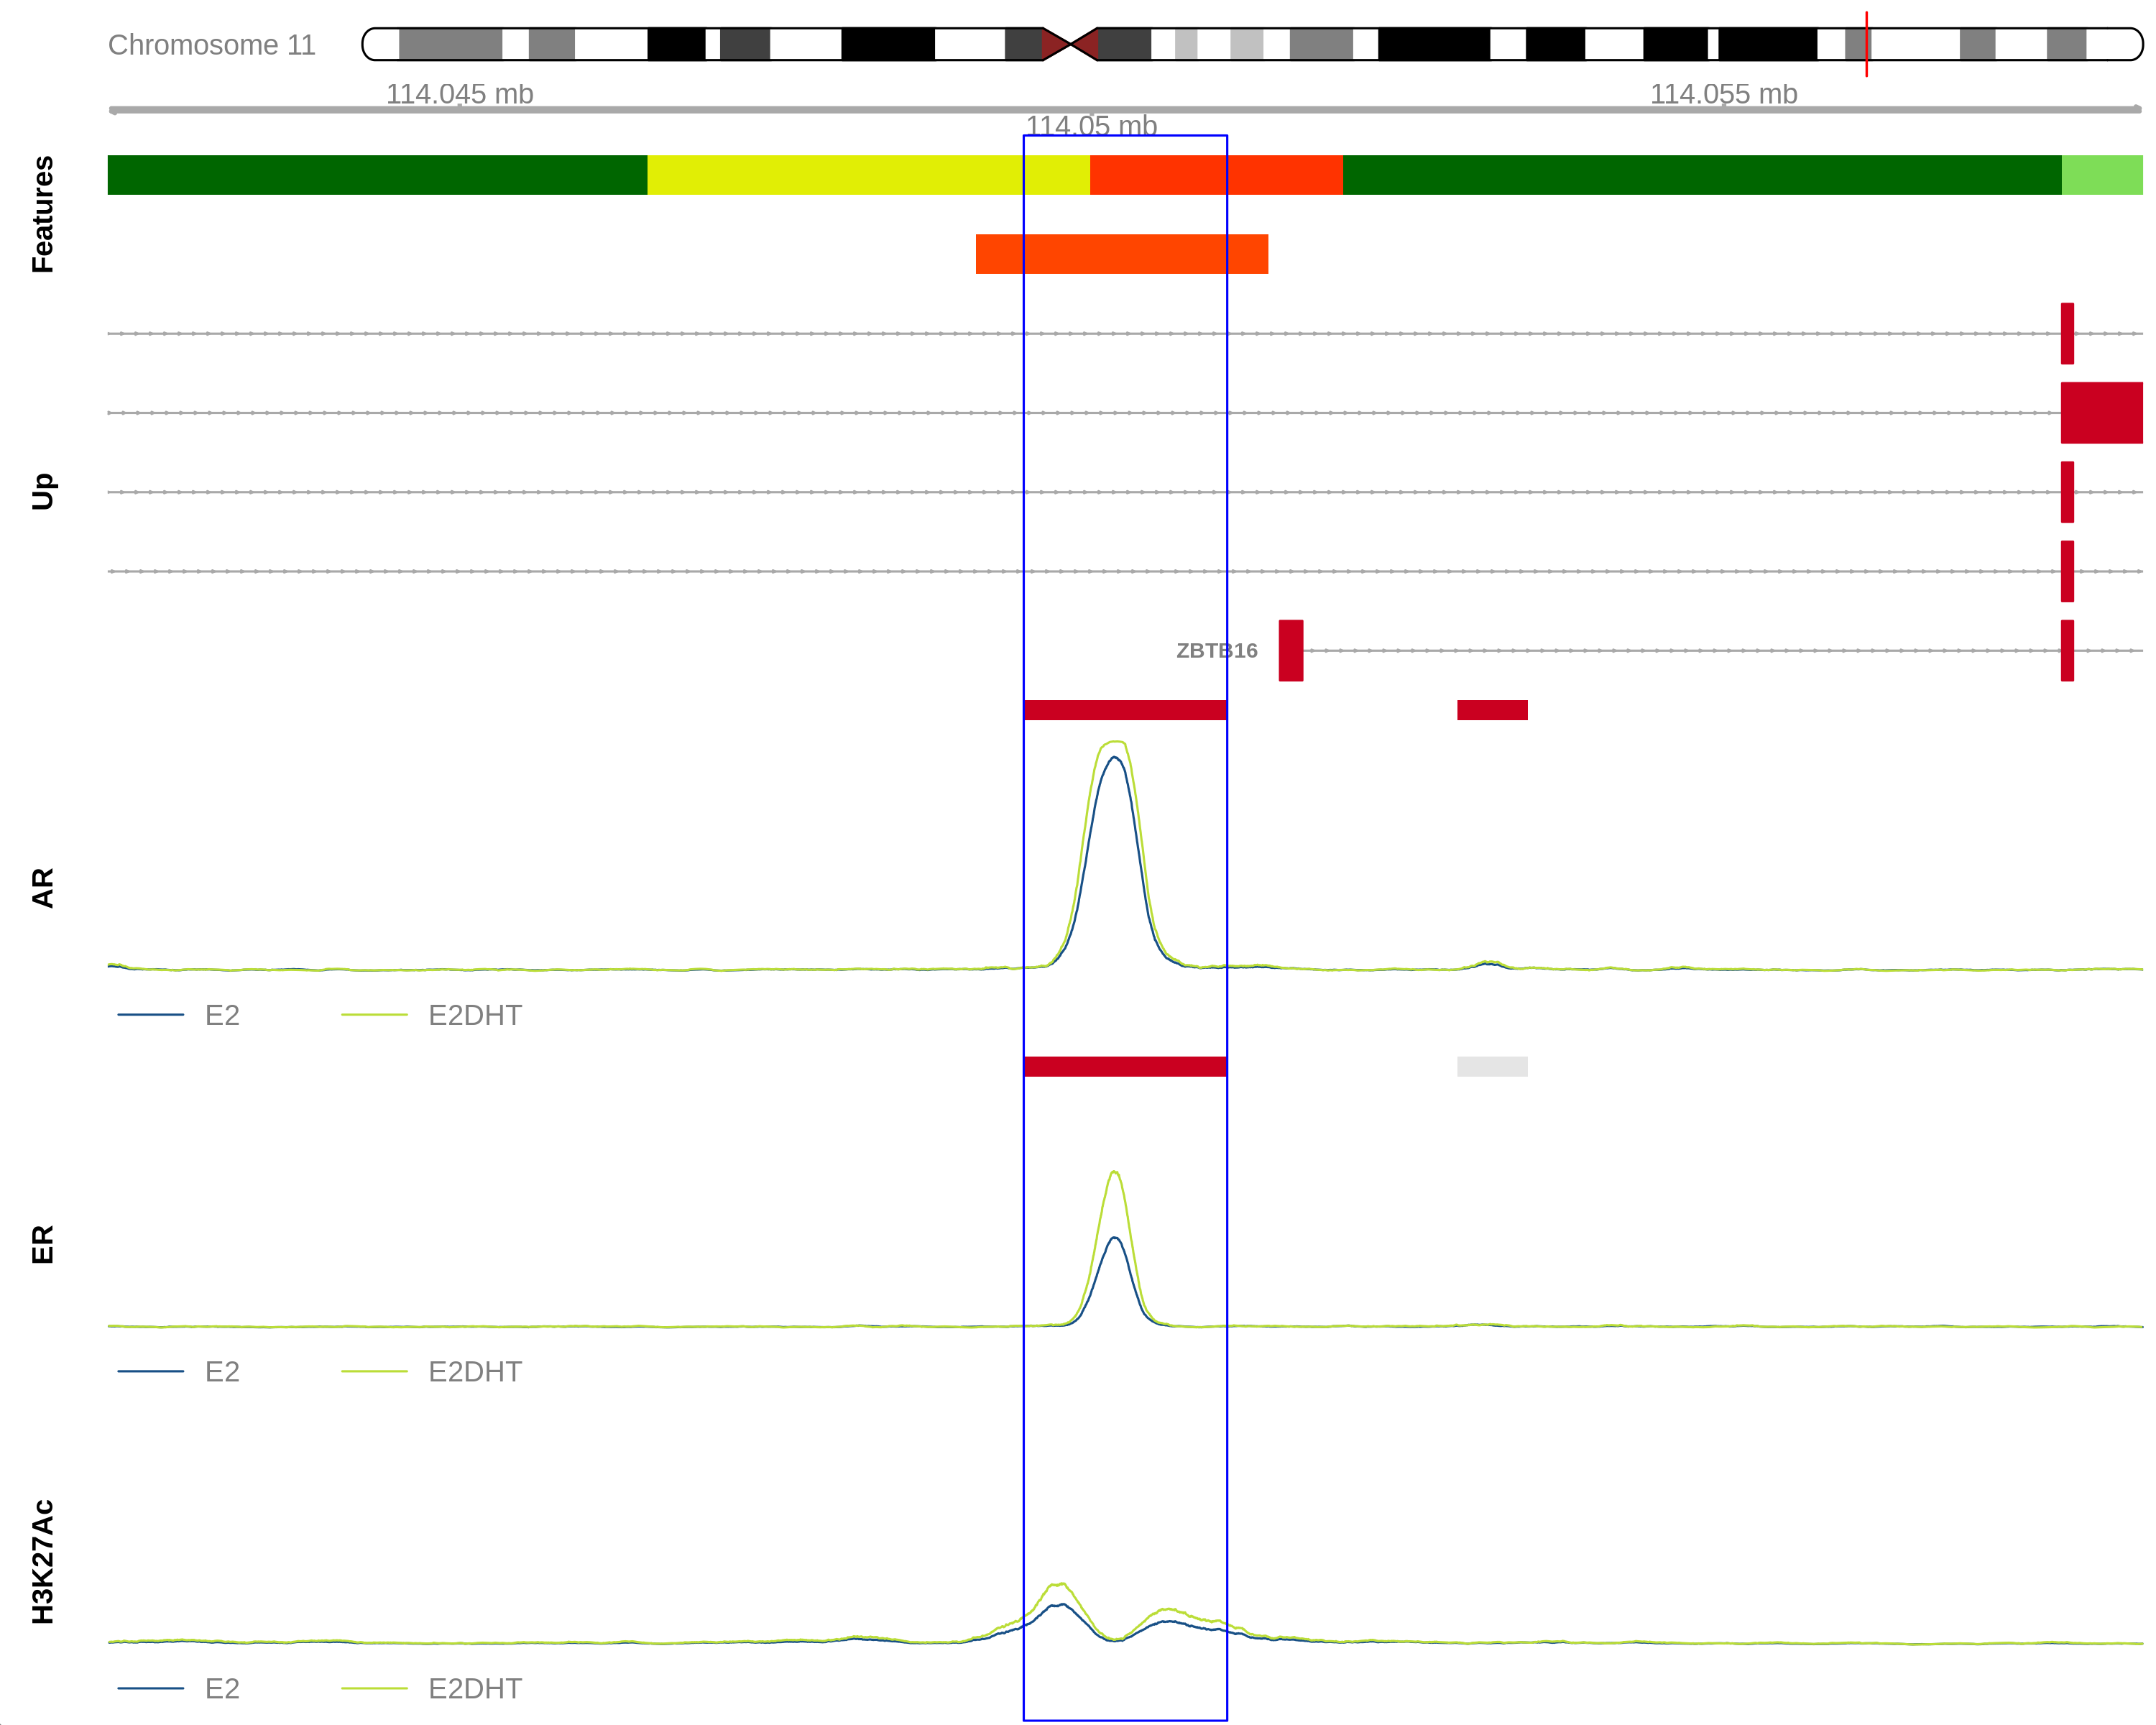
\includegraphics[width=0.8\linewidth]{AR_Up_ER_Up_AveExpr}
    	    \end{tikzfigure}		
		\end{minipage}
  		\begin{minipage}{0.5\linewidth}
  			\centering
           \begin{tikzfigure}[DE Genes by AR and ER binding patterns. Here, the top row would be the most informative.\label{fig:volcano}]
	        	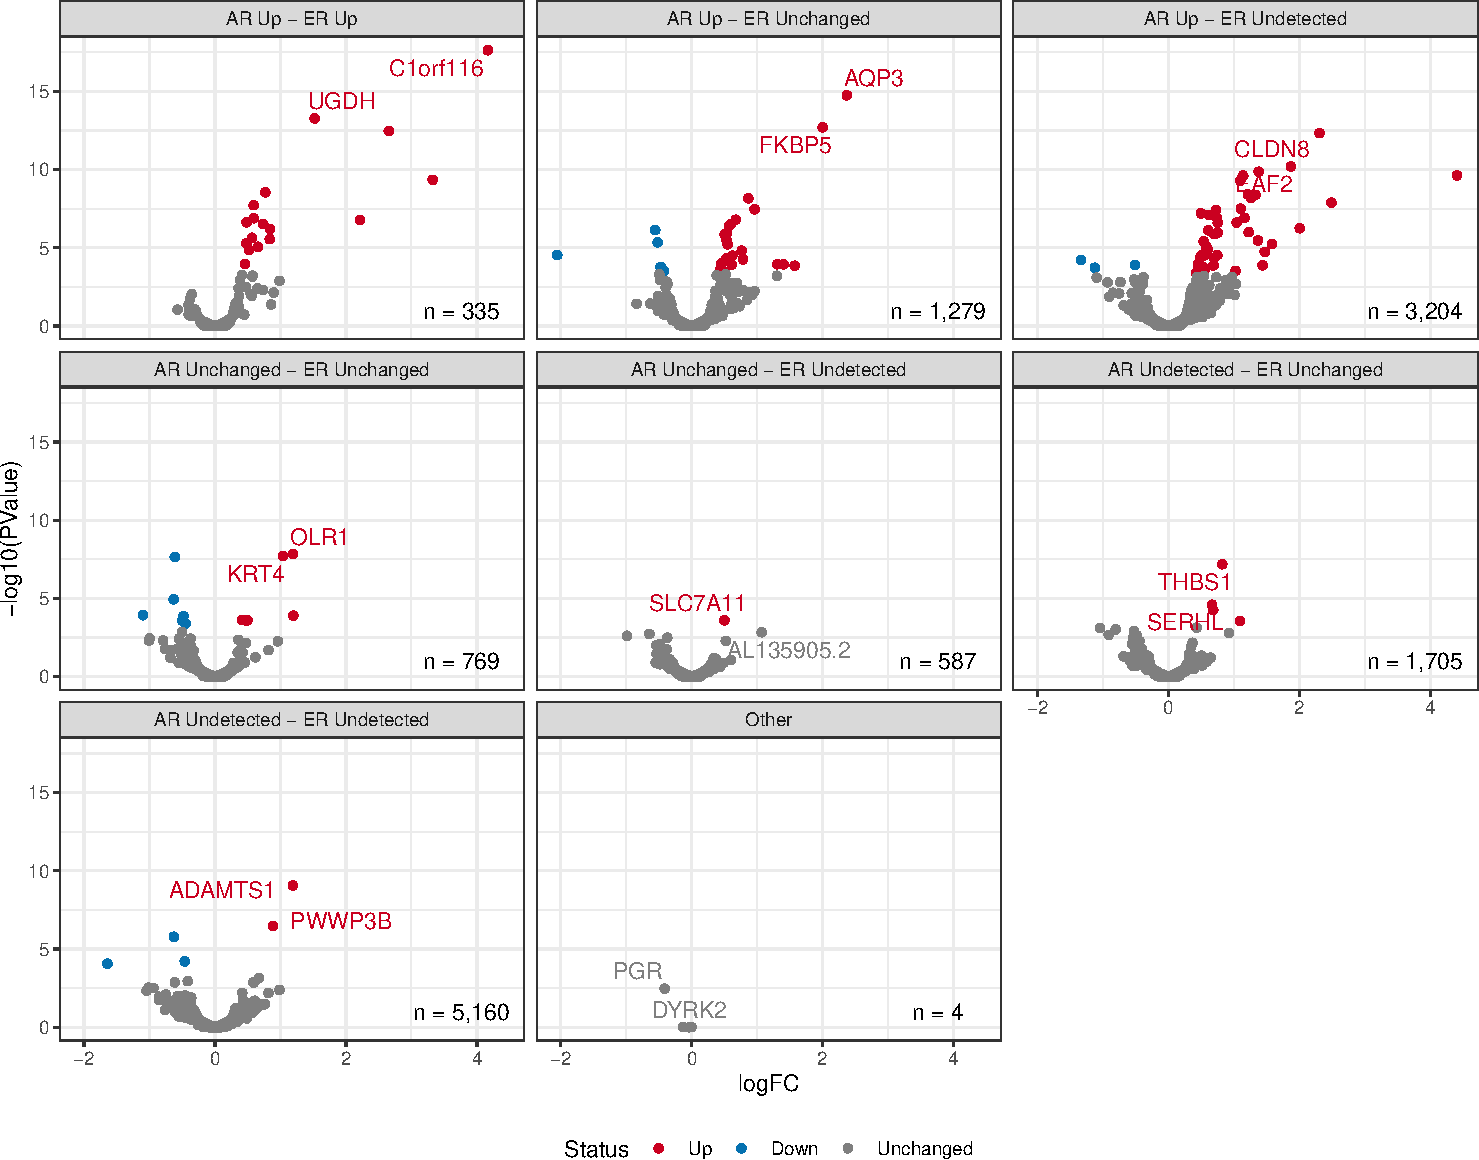
\includegraphics[width=0.82\linewidth]{plot-volcano-1}
    	    \end{tikzfigure}	
    	\end{minipage}\\[5mm]

    }
    
    
    \block{References}{
        \vspace{-1em}
        \begin{footnotesize}
        \printbibliography[heading=none]
        \end{footnotesize}
    }
\end{columns}
\end{document}